
Two primary motivations drive the exergy analysis done below.  The primary motivation behind this research is to demonstrate the differences in revenue generated between thermally and electrically coupling desalination systems to nuclear power plants in a NRHES configuration.   An additional motivation is \ac{aps}, which owns about 29\% of \ac{pvgs}, is evaluating electrically coupling a reverse osmosis system.  The \ac{ro} system will allow Palo Verde to fluctuate the amount of electricity sent to the electric grid while generating water to meet the power plant's own water requirements in addition to increasing the water resources available for communities in the surrounding region.

Due to its high penetration of solar energy, Arizona is an ideal setting to try a NRHES. Arizona has been a leader in implementing solar electricity. In 2013, Arizona produced 23.4\% of all US solar generation and 1.9\% of the electricity within the state.  By 2016, solar in Arizona nearly doubled production to 3.4\% of the total electricity for the state. The state also has a renewable portfolio standard requiring 15\% renewable energy by 2025 from regulated utilities\cite{DSIRE2017}. With an increasing penetration of solar in the state, other sources of generation will have to to be more flexible.

The Palo Verde generating station generates more electricity than any other power plant in the entire United States. In January 2018, Palo Verde produced 36.37\% of Arizona's power\cite{eia2018}.  As such a large contributor to the grid, Palo Verde fluctuating could counterbalance the large shifts in solar power generated during the day and unavailable during the evening and night hours. Palo Verde has a zero discharge water cycle.  Zero discharge means that, unlike most nuclear power plants that release heated water into a body of water, all of the water at Palo Verde either stays at the power plant forever or is evaporated from the evaporation ponds or the cooling towers.  The power plant uses waste water from Phoenix's 91st avenue treatment facility and Tolleson's water treatment facility. At the time of Palo Verde's initial operation in 1986, the treated waste water was not worth very much, but with the increasing unavailability of water and population growth in Arizona, water has become more valuable\cite{Brown2018}.  Arizona has significant amounts of brackish groundwater that could be pumped up from underground aquifers and used in place of the treated waste water currently in use at Palo Verde. The general composition of Arizona's brackish groundwater can be seen in Table\ref{ArizonaWater} below.

\begin{table}[h!]
\centering
\caption{The Components of Briny Groundwater in Central Arizona Centerra Well from \cite{USBureauofReclamation2006}}
\label{ArizonaWater}
\begin{tabular}{|l|l|}
\hline
\textbf{Material}                                                & \textbf{Mole Percent} \\ \hline
Calcium  & 7.32E-3     \\ \hline
Magnesium & 5.11E-3      \\ \hline
Sodium & 3.24E-2\\ \hline
Sulfate & 9.47E-3 \\ \hline
Barium & 5.25E-6 \\ \hline
Nitrate & 5.20E-4 \\ \hline
Flouride & 6.64E-5 \\ \hline
Arsenic & 7.21E-8 \\ \hline
Water                                                      & 99.9         \\ \hline
\end{tabular}
\end{table}

Palo Verde is pursuing a water purification facility in order to ensure a reliable and cost effective source of water for the power plant while also providing the surrounding communities with sufficient water to sustain growth. While Palo Verde is planning an electrically coupled reverse osmosis system, it is worth knowing what kind of water output would be expected from a thermally coupled system for future plants interested in pursuing desalination and water purification. Having six separate owners has led Palo Verde in the direction of an electrically coupled \ac{ro} system. \ac{aps} is the group considering the reverse osmosis system.  Since APS owns about 29.1\% of the facility, it owns about 29.1\% of the load generated from the facility. \ac{aps} has a total entitlement of 1146 MW from Palo Verde \cite{PinnacleWestCapitalCorporation2016}. APS can allocate the electrical load it owns as desired to the \ac{ro} system in order to fluctuate the electric load it sells to the grid as well as to ensure lower costs of water for the power plant. Even if using waste heat, thermal coupling to a reactor would impact the power cycle of the plant, as discussed in the results below. There are six owners of the \ac{pvgs}.  By thermally coupling any industrial process to a nuclear power plant, there will have to be some changes in the power cycle.  To have sufficient heat for even a low temperature process, some heat will have to be taken away from power generation. To avoid the complications of determining the technical as well as policy implications of thermally coupling with six owners, APS is opting for simplicity by pursuing an exclusively electrically coupled system \cite{Brown2018}.  Palo Verde demonstrates the restrictions imposed by the costs of increased complexity of thermal coupling. Coupling Palo Verde to a water purification system has multiple benefits.  One of the primary benefits is load following by sending excess power at times when electricity is cheap to produce clean water. The system could allow optimizing the value of the exergy lost in the system. Finally, by \ac{aps} owning the means of water production, the cost of water would be easier to predict and reliable. 


The literature review presented at the beginning of this thesis on NRHESs revealed a notable gap in the current research modeling the benefits gained from thermally coupling compared to electrically coupling industrial processes. Thermal coupling refers to using the heat directly from the nuclear power plant in industrial processes as opposed to generating electricity, which is then used by industrial processes. Fully determining the benefits of thermal coupling requires complicated analyses that are beyond the scope of this research. The full answer requires situated research focused on particular projects and includes economic, technical, as well as political and cultural factors. The goal for this research is to address some of the possible thermodynamic and economic benefits of thermally coupling nuclear power to industrial processes at a high level. 

The major drawbacks of thermally coupling any industrial process to a nuclear power plant are the increase in system complexity and the lack of experience in the domain. While there are cases of thermal coupling of nuclear power plants internationally; in Norway, Switzerland, Germany, and Canada \cite{Verfondern};  nuclear thermal couplings have never been used in the United States.  The low state of development as well as the lack of experimental data in the United States has created a lack of data and maturity of experience as a base for building such systems.  The uncertain regulatory environment regarding thermally coupled NRHESs and whether they fall under the \ac{nrc}'s umbrella also discourages development. 

The success of thermally coupled systems requires that their efficiency benefits be greater than the costs associated with developing and operating thermal coupling nuclear generation and co-locating industrial processes.  An exergy analysis of both the electrically coupled and thermally coupled industrial processes provides a quantitative measure of the thermodynamic benefits of thermally coupling. The fuzzy AHP analysis concluded that, given the characteristics of safety, ability to fluctuate, and profitability, the optimal industrial process is desalination. Based on this analysis, the exergy evaluation will focus on two desalination systems.  The thermally coupled system in this analysis is \ac{msf} distillation, which will be compared to an electrically coupled \ac{ro} system. The research concludes that, while thermally coupling is often thermodynamically better, electrically coupling results in greater revenue, given the assumptions built into the model.  

\section{Exergy Analysis Background}
% * <r.angelo.borrelli@gmail.com> 2018-06-12T21:22:56.058Z:
% 
% > Exergy Analysis Background
% Do you think it would be more instructive to include math representations of the 1st and 2nd laws?
% 
% ^.
The concept of exergy is helpful for analyzing the energy allocation in a system. Exergy, also known as availability, describes the energy available in the system for doing work. Exergy has the same units as energy, most commonly Joules. Exergy destruction occurs when energy is either used for doing work or through inefficiencies in the system.  By evaluating where exergy is destroyed and the economic value the product of the exergy destruction, in this case either electricity or clean water, a hybrid energy system can be optimized for revenue. 

Exergy describes the useful energy in a system for generating work. The first and second laws of thermodynamics clarify that not all the energy generated in a system can be converted into usable work.  The first law describes how energy cannot be created or destroyed, it can only be converted into a different form.  For example, chemical combustion in a fire produces heat and light. The second law states that entropy can only increase in a system. Entropy is often thought of as the amount of randomness in a system.  Having disorder or randomness in a system requires energy that cannot be used to generate work. Some energy always goes towards the entropy in the system, making it unusable, for example, to produce electricity. 


Exergy can be a more descriptive metric than energy loss as it describes how close a system is to an ideal design with the least physical possible energy losses across the system. In order to determine the maximum possible energy efficiency of a power cycle requires finding the Carnot efficiency $\eta_{Carnot}=1-\frac{T_0}{T}$. The Carnot efficiency finds the ideal possible output of a system. It is physically impossible for the Carnot efficiency to equal 100\%, which would be a perpetual motion machine.  Any system will always lose energy through entropy. The exergy efficiency describes the energy available to do work, how effective the cycle is designed to extract all of the available energy. The exergy analysis in this research evaluates the exergy lost in the power cycle as well as the exergy lost when using the pumps. The exergy analysis can then be combined with an economic analysis determining where exergy losses are most costly. For this project, the exergy analysis will include the components modeled in Palo Verde's Rankine Power Cycle as well as the water purification systems.

In an ideal reversible process, no exergy would be lost or entropy generated. Reversible processes are rightly named as these ideal processes could be restored to their initial state, the process reversed, without any external work added to the system. No processes are fully reversible in reality, since they would require that electric flow through a zero resistance material. Irreversible processes increase the entropy in the system, thereby removing some of the exergy in the system. Finding where exergy is destroyed in a system can help indicate where losses are occurring. By applying an economic exergy analysis, the system can be optimized so that the exergy losses are done in the most valuable way possible.
% * <r.angelo.borrelli@gmail.com> 2018-06-12T21:31:13.692Z:
% 
% > By applying an economic exergy analysis, the system can be optimized so that the exergy losses are done in the most valuable way possible.
% This makes it sound like the loss is most valuable. You mean 'minimal loss'?
% 
%There will be exergy losses in generating water and generating electricity. The exergy analysis focuses on making these losses valuable.
%
% ^.

The basic mass exergy equation of a system is\cite{moran2010fundamentals}:

\begin{equation}
\triangle X=(U-U_0)+p_0(V-V_0)-T_0(S-S_0)+KE+PE
\end{equation}
\\
Where X is the exergy of the system in kJ, U is the internal energy of the system in kJ, $p_0$ is the initial pressure of the system in kPa, $V$ is the volume of the system in $m^3$, $T_0$ is the initial temperature given in Kelvin, S is the entropy of the system in $\frac{joules}{kelvin}$, and KE and PE are the kinetic energy and potential energy in joules. The specific exergy of the system, or the exergy of the system not including the mass, is displayed as e.  To find the specific exergy of the system, each of the elements in the equation is divided by the mass which is in kg in this case. Specific thermodynamic properties differ from mass thermodynamic properties in that the specific values are characteristics of the materials regardless of mass. The resulting equation for internal exergy is:

\begin{equation}
\label{specificX}
\triangle x=(u-u_0)+p_0(v-v_0)-T_0(s-s_0)+\frac{1}{2}v^2+gh
\end{equation}
\\

The elements now represent the specific values of the system with the same units as above but per unit mass as opposed to the mass dependent variables shown in equation 3.1.  For this research, the mass values will be neglected, focusing instead specifically on the internal exergy values. The internal exergy differences thoroughly describe the system.  The mass transfer within either the power cycle or the water purification systems does not provide any extra insight into the relative magnitude of exergy loss in the various components. The kinetic energy term, $\frac{1}{2}v^2$, is generally fairly constant throughout the system and, therefore, does not need to be taken into consideration.  The potential energy element, $gh$, is negligible throughout the system. The enthalpy, h, of a system, or the total heat content of the system, is equivalent to the specific internal energy plus the pressure times the change in specific volume.  Put mathematically:

\begin{equation}
\triangle h=(u-u_0)+p_0(v-v_0)
\end{equation}

Including enthalpy in the place of the first two elements in equation \ref{specificX} as well as removing the last two elements leaves the specific exergy equation, which will be used in this research, as simply:

\begin{equation}
\triangle x=(h-h_0)-T_0(s-s_0)
\end{equation}

\subsection{Relevant Exergy Analysis Research}
Boldon et al. have already performed an initial exergy analysis on a \ac{nrhes}, assuming a \ac{smrs}\cite{Boldon}. Boldon et al. discuss the value of combining exergy and economics to analyze costs associated with exergetic losses. The assumptions in the Boldon et al. paper include a steady state system with a constant grid output of 245 MWe.  The nuclear plant is both thermally and electrically coupled to a High Temperature Steam Electrolysis industrial process. After performing the thermodynamic exergy analysis, Boldon et al. incorporate costs of resources and operations, enabling them to assign an exergetic unit cost to each of the components in the system. 

The exergy analysis in this paper differs from Bolton et al. by analyzing a current large nuclear power plant, by focusing on water purification methods, and by including a quasi dynamic approach.  While the value of the electricity and water will be taken into account, the products of the system will dictate the \$/exergy loss as opposed to the costs of the system. In order to include a quasi dynamic approach, both the MSF and RO systems will be evaluated based off of the optimal \$/exergy costs and will also take into consideration the load following capabilities valuable to \ac{aps}.

 An exergetic analysis of the Kalundborg industrial ecosystem, a non nuclear hybrid energy system, evaluates the streams going into and out of the Asnaes power plant \cite{Valero2012}.  Valero et al. contrast the exergy of the coupled system with an uncoupled system. As can be seen in figure \ref{Kalendburg} below, the Kalundborg industrial ecosystem is comprised of the Statoil refinery, the Asnaes coal power plant, the Novo Group pharmaceutical company, district heating for local residents, the Gyproc plasterboard manufacturer, as well as a fish farm and the Aalborg Portland cement company. The major exergetic gains for the system come from sharing process heat from the natural gas from the refinery, district heating, heating the fish farm, and using clinker (a coal plant byproduct) to produce cement \cite{Valero2012}. The overall reduction in irreversibilities annually from coupling the systems at Kalundborg amounts to approximately 1476 GWh/year, the equivalent of the annual production of a 170.235 MW power plant. By comparing the exergy of a coupled system with the separate industrial processes, the Kalundborg example provides insight into the thermodynamic and economic benefits of co-locating processes. Figure \ref{Kalendburg} displays the two different approaches taken; first evaluating the exergy of the combined systems, then evaluating the separate processes.

\begin{figure*}
\centering
\label{Kalendburg}
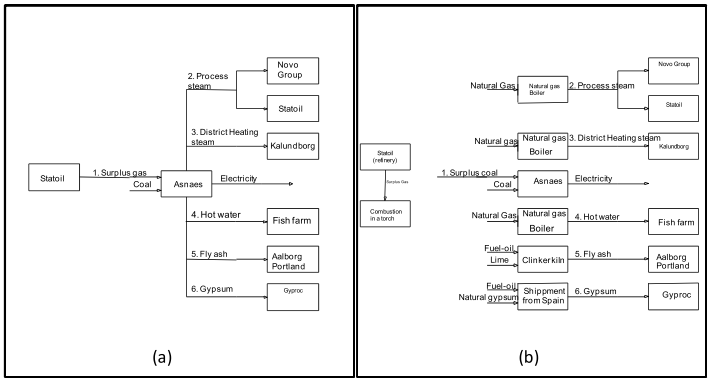
\includegraphics[width=.7\textwidth]{kalundborg_cases.PNG}
\caption{\small \sl This figure displays the two cases evaluated in Valero et al. Figure a shows the industrial ecosystem in the current coupled form. Figure b shows the second case where there is no coupling.}
\end{figure*}


\subsection{Multi-Stage Flash Distillation}
As the NRHES evaluated for this thesis includes a \ac{msf} distillation system, a brief review of a MSF distillation exergy analysis helps describes previous work done in this area. Kahraman et al. performed an exergy analysis on a large MSF plant \cite{Kahraman2005}.  \ac{msf} distillation only requires heat ranging from 80 to 120 degrees Celsius, making it possible to use high temperature waste heat from a nuclear power plant to desalinate or purify the water. In general, the waste heat coming from a nuclear power plant is significantly below 100\degree C. Extra heat would thus need to be sent to the environment, in this case the MSF process, in order to use the waste heat from the reactor. The same processes, RO and MSF, can be used for both water purification and desalination, so the terms can be used fairly interchangeably. In the case of Palo Verde, the system is a water purification system for brackish groundwater. In the exergy analysis, Kahraman et al. takes the temperature of the salinated water to be the dead state, or the assumed initial conditions for the systme, making the initial exergy zero. Similarly, in the exergy analysis done in this thesis, the dead state is taken as the temperature of the water intake. Kahraman et al's exergy analysis includes finding the exergy of the heat exchanger and four pumps in the system, as well as calculating the difference in exergies between the incoming water and the exiting stream.


Figure \ref{MSF_x} displays where exergy was destroyed in the MSF system. Clearly the majority (77.7\%) of the exergy was destroyed in the MSF distillation system itself. Other sources of irreversibilities include the inefficiencies and losses due to the pumps and heat exchangers as well as the final release of the waste brine water to the environment. The exergy destroyed in the MSF system went to a process that produced a valuable product.  The other sources of exergy destruction are physically necessary losses with no economic benefits. In the economic exergy study done in this thesis, the exergy destruction will be evaluated based on its economic value.  Both generating pure water in the MSF system as well as producing and using electricity for the reverse osmosis system result in exergy destruction.

MSF is a common thermal desalination system, making up about 21\% of the total worldwide installed capacity. In an MSF system, salt water or brackish water is flash evaporated, then condensed repeatedly in order to remove unwanted particulates. As can be seen in figure \ref{salinity}, brackish water has more salinity or impurities than fresh water, but not as much as sea water. MSF can produce clean water in large quantities, with plants in Saudi Arabia and the United Arab Emirates having capacities of 600,000-880,000 $m^3/day$ \cite{El-Dessouky2016}. In general, an MSF system works by passing sea water or briny water through a series of chambers, each with successively lower temperature and pressure.  The water is quickly flashed, or vaporized.  The water, without the brine, is then condensed, forming freshwater.  The stages can range widely, depending on the concentration of the feedwater brine and the desired state of purity for the freshwater. Standard sizes for fairly large MSF arrays range from 21 to 50 stages. Generally, MSF distillation systems are a well-developed technology used for high capacity desalination systems.
\begin{figure*}[h!]
\centering
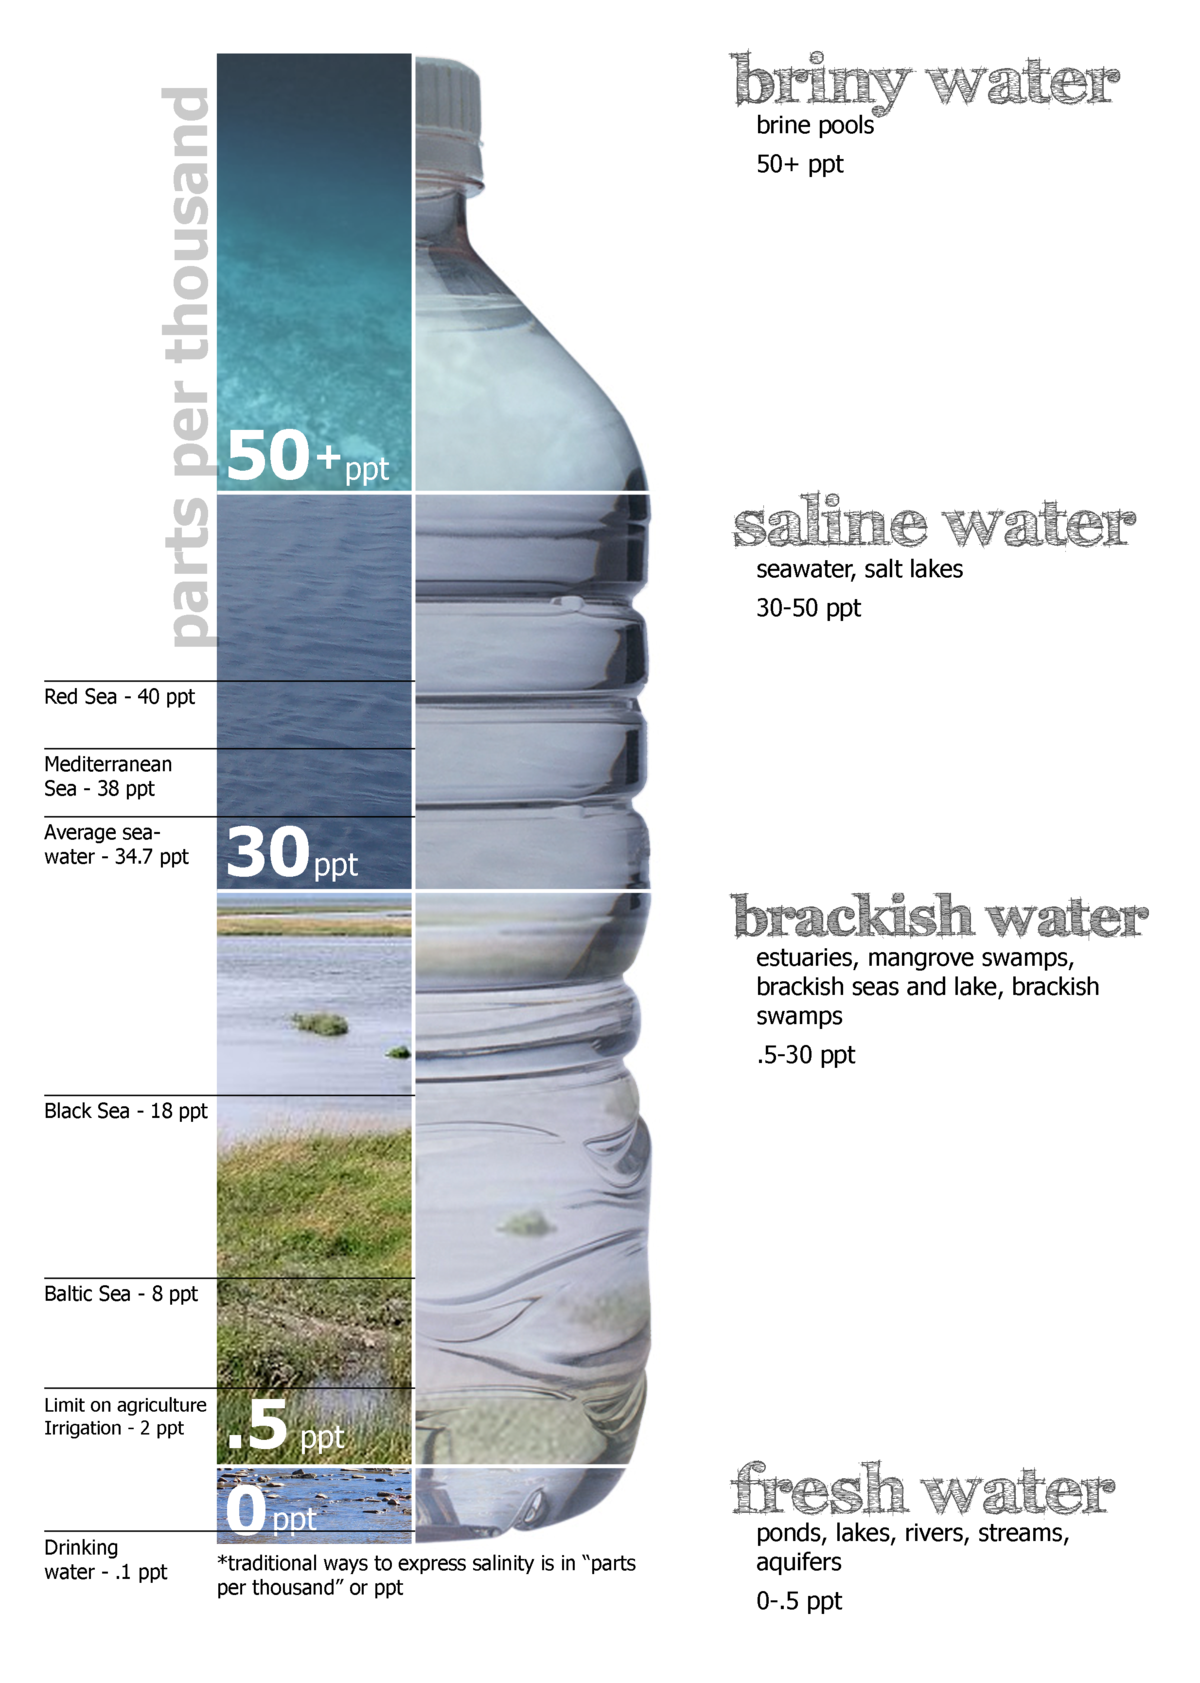
\includegraphics[width=.25\textwidth]{Water_salinity_diagram.png}
\caption{\small \sl This figure displays the differences between different water qualities}
\label{salinity}
\end{figure*}


In a multi-stage flash system, it is important to keep the temperature relatively low, no greater than 120 \degree C, in order to minimize fouling. Fouling and scaling are serious considerations for MSF systems.  Generally, fouling refers to the unwanted deposition of compounds or organic substances on the surface of a host material (membrane, heat exchanger, condenser, etc)\cite{Khayet2016}. Scaling is when a surface is entirely covered with a mineral film coating. In \cite{El-Dessouky2016} the twelve case studies range from 95 \degree C to 105 \degree C. For a more complete range of possible temperatures, this research will analyze temperatures from 80 \degree C to 120 \degree C.


\begin{figure*}[h!]
\centering

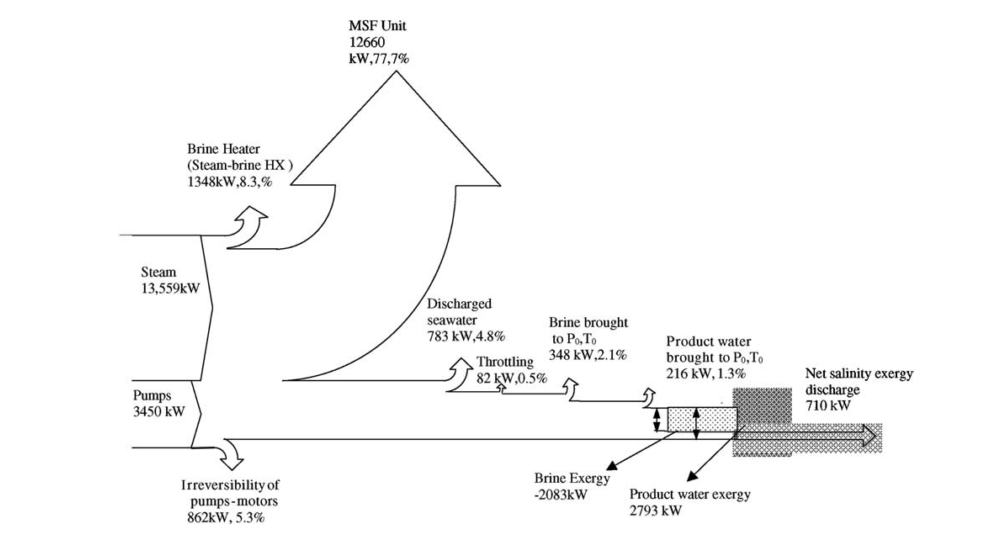
\includegraphics[width=.4\textwidth]{MSF_exergy.PNG}
\caption{\small \sl The Multi-Stage Flash exergy analysis diagram showing where exergy is lost in the system from \cite{Kahraman2005}}
\centering
\label{MSF_x}
\end{figure*}

\subsection{Reverse Osmosis}

Reverse osmosis is a type of electrically driven membrane desalination or filtration process. It can remove tiny particles of sizes ranging down to 50-200 daltons \cite{Pangarkar2011}. It has relatively high applied pressure values ranging between 1-5 MPa. In general, the reverse osmosis system works due to the osmotic pressure differences between salt water or briny water and pure water. During the \ac{ro} process, salt water or briny water is forced through membranes under pressure, separating the feedwater into a pure water stream and a stream with a high concentration of impurities.  About 48\% of reverse osmosis systems are used with brackish water \cite{Pangarkar2011}.

\begin{figure*}[h!]
\centering
\label{DesalData}
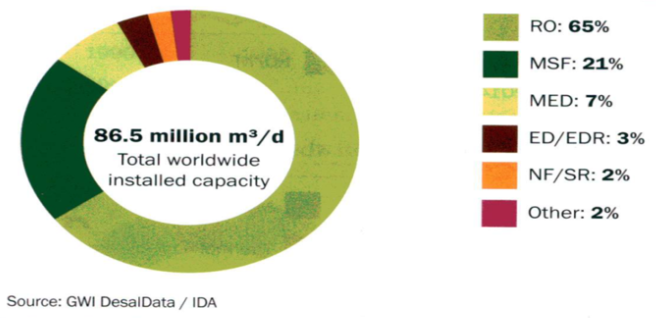
\includegraphics[width=.5\textwidth]{DesalData.PNG}
\caption{\small \sl This pie chart shows the overall total installed capacities of each of the technologies used for desalination.  This is taken from a not-yet presented presentation by Ibrahim Khamis to ANS, which I still need to get permission to use}
\centering
\end{figure*}

\section{Methodology}
 The exergy analysis done here will assume a simplified model of the Palo Verde Rankine power cycle, seen below in figure 3.5, and compare a process heat MSF distillation system to a RO system.  First, the  \$/exergy cost of an MSF system will be evaluated using the process heat from a nuclear power plant. Then the same process will be applied to the exergy costs of the RO system, which strictly uses electricity. An exergy analysis really evaluates where there are irreversibilities in a system. In order to show the irreversibilities in the system requires evaluating the exergy destroyed across each of the subsystems.  With the power cycle, the subsystems include the turbines, the heat exchangers, and the pumps.  The exergy change across the condenser is taken to be the exergy destroyed in order to purify the brackish groundwater. While some exergy left in the brackish waste water is released to the environment, the exergy destroyed through the condenser provides a general idea of how much exergy was required in the MSF system. In the case of the RO system, the exergy lost in the condenser is part of the exergy loss required for the electricity generation. The exergy losses in the RO system come strictly from the exergy destroyed in the pumps. The economic values for the system will come from the value of the electricity generated plus the value of the water generated.  


The system will be modeled using the Aspen HYSYS software.  The power cycle will initially be a simplified version of the Palo Verde Power cycle.  Since the goal in this research is to evaluate the differences in the water purification systems, not the exergy losses in the power cycle, the power cycle model primarily serves to demonstrate how thermally coupling a system impacts the system as a whole. The overall exergy lost is the same throughout the power cycle, the losses can generate either electricity or water.

\subsection{Aspen HYSYS}

Aspen HYSYS is process simulation software used primarily by the oil and gas industry. In general, process simulation software calculates material and energy balances for a whole plant or process unit. Process simulation software can be used to size the various components in a system for the desired outcome in terms of quality and quantity of product. Aspen HYSYS calculates heat and mass balances, thermodynamic data and equilibrium conditions, sizes equipment, and can do economic optimization and dynamic simulation \cite{Oi2017}. In this model, Aspen HYSYS calculates the overall thermodynamic and mass flow values of the Palo Verde Power Cycle as well as the multistage flash distillation process. The thermodynamic values, such as enthalpy, entropy, temperature, and pressure can then be used to determine the exergy of the system using a User Variable in the system.

First, as can be seen in figure \ref{basePC}, determining the exergy analysis required building the Palo Verde power cycle using Aspen HYSYS and coupled it to both a MSF and RO water purification systems. The configurations for the MSF and RO systems can be seen in figures \ref{MSF} and \ref{RO} respectively. After the building the model, in order to find  the \$/exergy in the power cycle and the water purification system required using a combination of user variables within Aspen HYSYS as well as spreadsheet calculations, as can be seen in Appendix B. Then, after finding the exergy values, in order to determine the optimal temperature of water required adjusting the temperature of the water sent to the heat exchanger with the MSF system.  

 \begin{figure*}[h!]
\centering
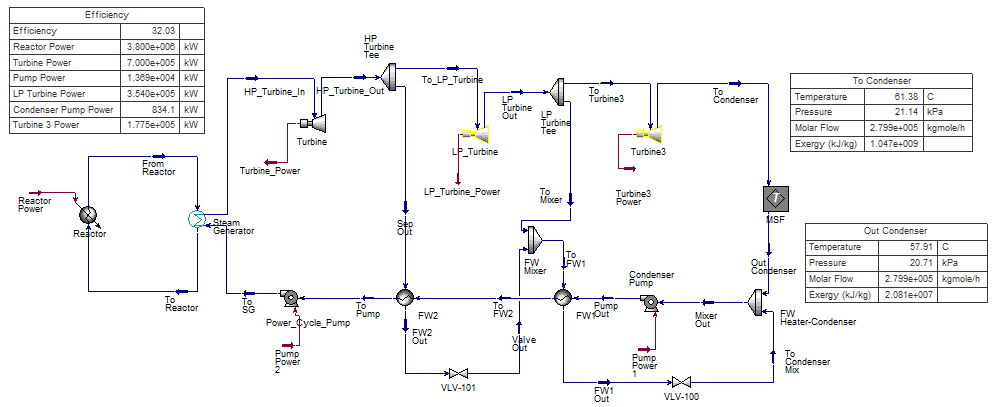
\includegraphics[width=.5\textwidth]{ActualPC.PNG}
\caption{\small \sl This is an image of Palo Verde's simplified Rankine cycle used for this research. The overall efficiency of the system is about 32\%, which is a reasonable approximation of the Palo Verde Power cycle.  The turbines are yellow, meaning warning, because of the liquid entering the turbines.  In reality, the turbines can still function with some liquid}
 \label{basePC}
\centering
\end{figure*}

\begin{figure*}[h!]
\centering

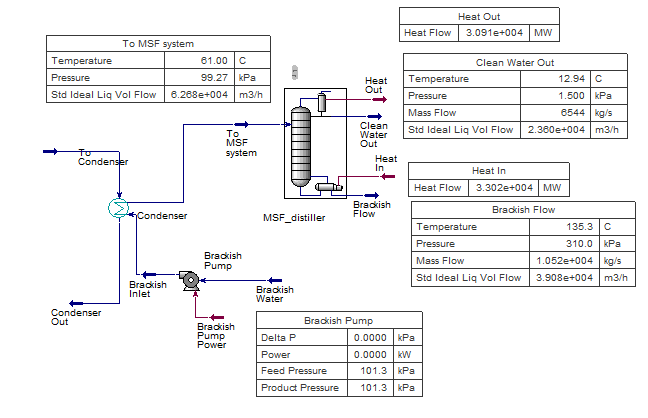
\includegraphics[width=.5\textwidth]{PowerCycle.PNG}
\caption{\small \sl This figure shows the distillation column used to represent the multi-stage flash system along with key important metrics for the various components.}
\label{MSF}
\centering
\end{figure*}

\begin{figure*}[h!]
\centering
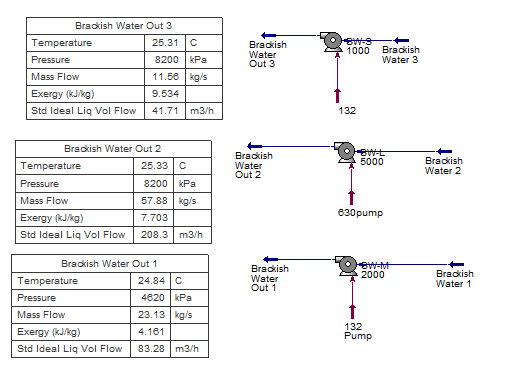
\includegraphics[width=.5\textwidth]{ROimage.PNG}
\caption{\small \sl The energy used for an RO system comes almost entirely from the pumps used.  The three pumps shown here represent off the shelf pumps used in Reverse Osmosis systems}
\label{RO}
\centering
\end{figure*}

Doing an economic analysis evaluating the \$/exergy requires knowing the amount of product sold as well as the value of the product. The cost of water for Palo Verde in 2018 is \$130.00 per acre-foot, which comes out to about \$0.105 per cubic meter of water \cite{Brown2018}. The water is very cheap.  For comparison, the residential cost of water in Tucson in 2017 was about \$1.42 per cubic meter \cite{CityofTucson2017}. The best value available for the wholesale value of Palo Verde's electricity is from 2007 at 6.33 cents per kWh, which is equal to about 8 cents per kWh including inflation. The actual value of the electricity fluctuates over a day depending on the supply of electricity. The actual wholesale sales price of electricity for Palo Verde is confidential information, so the price values are approximations.  In Arizona's case, the value of the electricity over the course of a day could be largely influenced by the amount of solar supply available to the grid. The fluctuation in power demand for \ac{aps} will be taken into consideration using \ac{raven} to generate demand data for a generic day in each season.

\subsection{Fluctuating Electricity Output}

In order to be considered by \ac{nerc}, a regulating and supplemental reserve of electricity requires that a non-spinning reserve source be able to ramp to full capacity within ten minutes \cite{NERC2014}. NPPs traditionally are unable to fulfill a role as regulating or supplemental reserve because of the inability to ramp to full power quickly.  With an MSF system, the NPP still may be unable to switch the process heat fast enough to meet the NERC's definition. The European Utility Requirements require that an NPP be capable of daily load cycling operation between 50\% and 100\%. The European pressurized water reactor must satisfy maneuverability requirements, including being able to have planned variations in energy output between 25\% and 100\% \cite{NEA2011}. For this research, the MSF process heat model will be evaluated at 25\%, 50\%, 75\%, and 100\% of the heat load from the reactor. Looking at 25\% intervals will give some notion of the relationship between the heat sent to the MSF system and the amount of water collected from the system.

\subsection{Drinking Water Standards}
Some water quality standards must be met to ensure the water produced by the purification is of high enough quality to use in Palo Verde's power cycle as well as to sell to the public. The main consideration for the water purification system, especially if planning on selling the water to the public, is that the water must meet the standards established by the Safe Drinking Water Act of 1974. While commercial nuclear power plants dedicate a lot of resources to water chemistry and have very high standards for the water used in the plant, the standard used for this research will be that set for public consumption. Below is a discussion of both the standards as well as the current composition of briny groundwater in Arizona.

The Safe Drinking Water Act of 1974 gives the \ac{epa} the authority to determine drinking water standards. The EPA sets standards on over ninety contaminants in drinking water. The drinking water contaminants fall into the broad categories of microorganisms, disinfection byproducts, disinfectants, inorganic chemicals, organic chemicals, and radionuclides \cite{USEPA}. The components found in Arizona groundwater can be found in table \ref{ArizonaWater}.  None of the components found in Arizona groundwater are regulated by the Safe Drinking Water Act or are covered by the EPA's secondary drinking water standards\cite{USEPA}. The only overlap between the contaminants regulated by the EPA for taste and aesthetic concerns and those found in Arizona groundwater is maintaining the total dissolved solids at 500 mg/L or below. For this research, the water is assumed to be comprised of a more brackish composition than that found in table \ref{ArizonaWater}. The contaminants have been increased nine fold in the composition used in the Aspen HYSYS model as can be seen in table \ref{ModelComp}.  In some cases, the independent materials found in the brackish ground water were unavailable in the Aspen library.  As a result, the model includes combined molecules, such as sodium sulfate and sodium nitrate to most closely proportionally match the composition found in the groundwater.  Combining these molecules may result in some difference in the overall composition and the energy it takes to remove the particulates. The end product is pure water.

\begin{table}[h!]
\centering
\caption{Mole Composition of Brackish Groundwater Assumed in Aspen-HYSYS model}
\label{ModelComp}
\begin{tabular}{|l|l|}
\hline
\multicolumn{1}{|c|}{\textbf{Material}}                   & \multicolumn{1}{c|}{\textbf{Mole Percent}} \\ \hline
Calcium & 1.3E-1 \\ \hline
Magnesium  & 9E-2\\ \hline
Sodium  & 5E-1 \\ \hline
Sodium-Sulfate & 1.7E-1 \\ \hline
Sodium-Nitrate & 9E-2 \\ \hline
Barium & 1E-2 \\ \hline
Water & 99.0  \\ \hline
\end{tabular}
\end{table}

\section{Palo Verde Power Cycle}

Much of the information of the design and functioning of Palo Verde's power cycle can be found in the \ac{ufsar}, made publicly available for all nuclear power plants by the \ac{nrc}. Some of the key values taken from Palo Verde's \ac{ufsar} are displayed in tables \ref{coreValues} and \ref{PowerValues}. The initial value given in FSAR is what the FSAR actually states.  The second value represents the converted value into the units used in the model of this thesis.  The key difference between the model values and the Main Steam Flow Power Cycle Values is the mass flow is significantly less for the model 1616 $\frac{kg}{s}$ compared to 2200 $\frac{kg}{s}$. The mass flow value is solved for in the model. As the thermodynamic values taken for this research are specific values that do not include the mass flow, the findings should be relevant to any mass flow. Overall, while the simplified Palo Verde Power Cycle does not precisely model the actual power plant, it has enough similarities to suggest some trends by the exergy analysis. Since not all of the components are included in the model, the lower mass flow calculated is to be expected. 
% * <r.angelo.borrelli@gmail.com> 2018-06-12T22:56:44.911Z:
% 
% > The key difference between the model values and the Main Steam Flow Power Cycle Values is the mass flow is significantly less for the model 1616 $\frac{kg}{s}$ compared to 2200 $\frac{kg}{s}$. 
% This isn't clear to me why there is a difference. 
% 
% ^.

There are two model configurations included in this analysis.  One of the configurations, as seen in figure \ref{MSF_condense}  draws water from the end of the power cycle.  As the Palo Verde Power Plant would want to minimize impact to the thermal hydraulics of the system, using the condenser and switching to passing groundwater through the system would allow for use of existing infrastructure. The second configuration, as can be seen in figure \ref{MSF_SG}, allows for a more efficient system that draws water straight from the steam generator at very high temperatures. Since the efficiency of the ideal Carnot cycle is very dependent on the change in temperature through the cycle, drawing water from the reactor initially allows for a greater drop in temperature throughout the cycle.  When taking a percentage of the water at the beginning of the power cycle, the water leaving the last turbine does not have to be a minimum of 80\degree C for the \ac{msf} system.  Also, water at 289.4\degree C can heat a lot of water at 24.44\degree C to 80\degree C. The second configuration would allow for differing amounts of water to be sent to the MSF as opposed to different temperatures of water as is the case when using the condenser as a heat exchanger for the MSF system.

\begin{figure*}[h!]
\centering
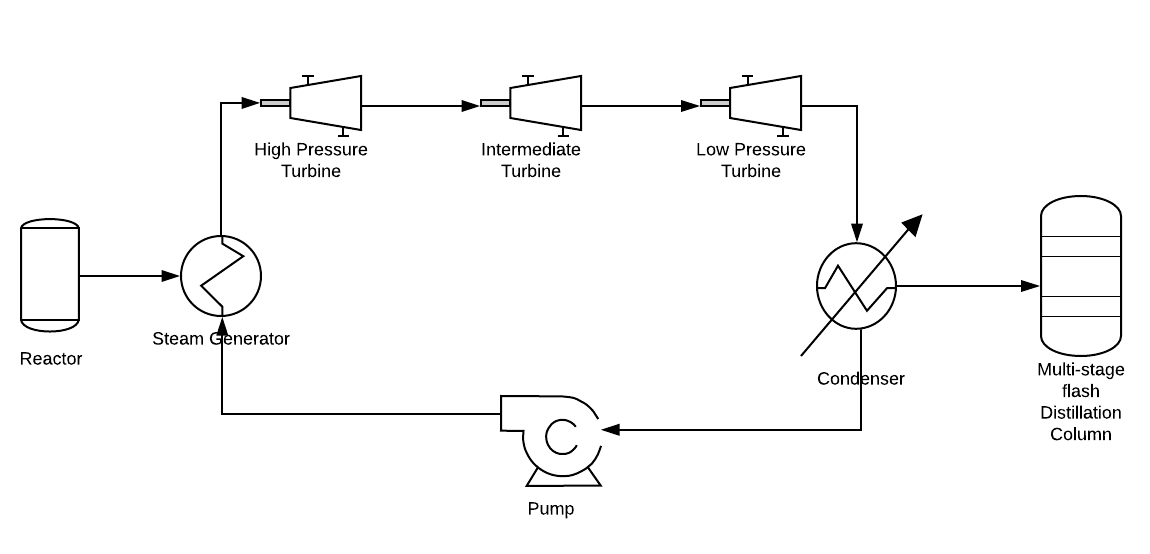
\includegraphics[width=.8\textwidth]{MSF_condense.png}
\caption{\small \sl This simplified drawing shows the main components of the power cycle including how the multistage flash distillation system is heated through the condenser}
 \label{MSF_condense}
\centering
\end{figure*}

\begin{figure*}[h!]
\centering
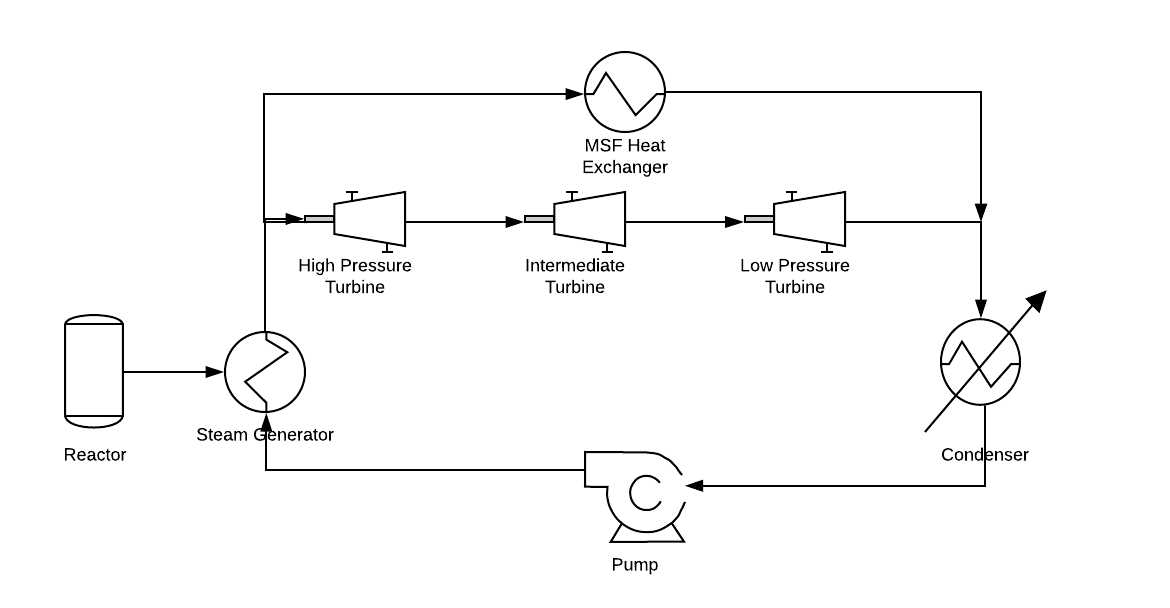
\includegraphics[width=.8\textwidth]{MSF_lucidchart.png}
\caption{\small \sl This simplified drawing shows the main components of the power cycle including how the multistage flash distillation system draws water just after the steam generator}
 \label{MSF_SG}
\centering
\end{figure*}

\begin{table}[h!]
\centering
\caption{Palo Verde Reactor Core Thermohydraulic Values. The first units given in the Value Given in FSAR column are the actual values found in the FSAR, while the second are the converted values into those used in the model.}

\begin{tabular}{|l|l|l|}
\hline
\textbf{Reactor Core Values} & \textbf{Value Given in FSAR} & \textbf{Value in Model}        \\ \hline
Reactor Outlet Temperature   & 653 \degree F, 345\degree C & 345 \degree C   \\ \hline
Reactor Inlet Temperature    & 568 \degree F, 297.8 \degree C &  297\degree C\\ \hline
Mass Flow                    & $164.0x10^6\frac{lb}{hr}$    & $20663.6\frac{kg}{s}$          \\ \hline
Pressure                     & 2250 psia, 15.513 MPa                    &  15.51 MPa                    \\ \hline
Power Generation             & 3990 MWt                     & 3990 MWt                       \\ \hline
\end{tabular}
\label{coreValues}
\end{table}


\begin{table}[h!]
\centering
\caption{Palo Verde Main Steam Flow Power Cycle.  The first units given in the Value Given in FSAR column are the actual values found in the FSAR, while the second are the converted values into those used in the model.}
\label{PowerValues}
\begin{tabular}{|l|l|l|}
\hline
\textbf{Power Cycle Values} & \textbf{Value Given in FSAR}  & \textbf{Values in Model}          \\ \hline
Steam Temperature at HX     & 552.9 \degree F, 289.4 \degree C &   289.4 \degree C                 \\ \hline
Mass Flow                   & $17.2-18.1x10^6\frac{lb}{hr}$, $2154.56-2280.56 \frac{kg}{sec}$ & 1616 $\frac{kg}{sec}$ \\ \hline
Pressure & 1070 psia, 7.377 MPa  &   7.377 MPa                     \\ \hline
\end{tabular}
\end{table}


\subsection{Assumptions}
% * <r.angelo.borrelli@gmail.com> 2018-06-12T23:04:30.088Z:
% 
% Where did this come from?
% 
% ^ <r.angelo.borrelli@gmail.com> 2018-06-12T23:04:54.202Z.
% * <r.angelo.borrelli@gmail.com> 2018-06-12T23:03:07.257Z:
% 
% > Assumptions
% You might want to note if you're pulling values from the FSAR. 
% 
% ^.

Given the information above, the assumptions for both the \ac{msf} and \ac{ro} Aspen HYSYS models are:
\begin{enumerate}
\item The temperature of the brackish groundwater entering the system is 76 \degree F or 24.44 \degree C, the low end of the temperature range for the water currently used to cool the system \cite{Brown2018}. Groundwater would be colder, but sitting in a pool above ground would raise the temperature. The assumption of the water being at the low end of what currently flows through the condenser allows an analysis of using the groundwater and also allows for a fair comparison of the MSF and RO systems using the most realistic value for both.
\item The reactor power, as is given in the FSAR, is 3990 MWth
\item The temperatures for the MSF distillation unit range from 80 \degree C to 120 \degree C
\item The composition of the water is what is shown in \ref{ModelComp}
\item There is a 2\% pressure loss across all heat exchangers
\item The turbines in the Palo Verde power cycle have a 90\% adiabatic efficiency
\item The pumps have a 90\% adiabatic efficiency.
\item The fluid package used for the power cycle was Peng-Robinson, which is the fluids package with the largest applicability range for temperature and pressure.
\item The fluid package used for the brackish water was Aspen's Electrolyte NRTL. This fluid package is especially good for modeling all of the various components in the brackish feedwater composition.
%Explain what this means
\item The power cycle is much simplified in order to show the clear impacts of the different water purification techniques as opposed to emphasizing the power cycle itself.
\end{enumerate}

The assumptions for the MSF Aspen HYSYS models are:

\begin{enumerate}
\item There are twenty one stages in the MSF distillation system \cite{Bodalal2010}
\item The mass flow through the distillation system is the dependent variable while the temperature of the water sent to the unit and the pressure generated from the briny water pump are the independent variables for the MSF system.
\item The reactor power and electricity produced are independent variables.
\item The temperature of the water sent to the condenser is an independent variable.
\item The pump power is a dependent variable.
\item The electric power generated is the independent variable.
\item The amount of water generated and the electricity generated are the dependent variables depending on the desired temperature of water sent to the condenser.
\end{enumerate}

The assumptions for the RO Aspen HYSYS model are:

\begin{enumerate}
\item The efficiency of the pumps ranged from 70\% to 80\% depending on the specifics of the expected pressure and water outflow given by the company
\end{enumerate}

The economic assumptions for all Aspen HYSYS models are:
\begin{enumerate}
\item The cost of water for Palo Verde Generating Station is \$130 per acre foot \cite{Brown2018}
\item The wholesale price which Palo Verde can sell water to the grid is \$.08 per kWh.
\end{enumerate}

The simplified Aspen HYSYS model includes one high pressure and two low pressure turbines.  The three separate turbines allow for one of the turbines to be taken offline independently to send higher temperature water to the MSF system. To find the \$/exergy values, required the following calculations:

Found the electricity revenue by multiplying the electricity produced by the system in MW by the wholesale electricity price per MWh, assumed by this research to be \$80 per MWh:
\begin{equation}
Electricity\hspace{.2cm} Revenue=MW_{out}*\frac{\$80}{Mwh}=\frac{\$}{hr}
\end{equation}

To find the water revenue, required multiplying the water produced by the system by the wholesale value of water to the Palo Verde Generating Station to find the hourly value of the water
\begin{equation}
Water\hspace{.2cm} Revenue=\frac{m^3_{out}}{hr}*\frac{\$.105}{m^3}=\frac{\$}{hr}
\label{water}
\end{equation}

%When lower temperatures, such as the 80\degree C example, were sent to the \ac{msf} system, the system did not have enough heat to clean all the water passing through the condenser.  In these cases, heat had to be added to the \ac{msf} system. To find the cost of the heat added to the distillation system for the lower water temperature studies required using the hourly value for electricity, multiplied it by the efficiency of the system, then multiplied by the heat required by the distillation columns.  This is an imperfect calculation, as the heat value is then based on both the efficiency of the cycle and the cost of electricity.  The heat would have to come from a separate source, either through electricity conversion or more direct heat.  Likely in these circumstances, the added expense of thermally coupling several processes would be unrealistic and the cost of the heat would be too high.  The examples that include a demand for extra heat for the MSF system are essentially negligible.  They are included in this study to demonstrate the full range of values that research suggests are possible with MSF.  There might be a way to produce less water with the heat sent to the distillation system, but that research is beyond the scope of this project.  
The equation used to find the value of the heat added to the MSF distillation system is:

\begin{equation}
Water\hspace{.2cm} Heat \hspace{.2cm} Cost=\frac{\$}{MWh}*Efficiency*Heat \hspace{.2cm}Required  \hspace{.2cm} by  \hspace{.2cm} MSF=\frac{\$}{hr}
\end{equation}

To find the \$/exergy destroyed:

\begin{equation}
\frac{\$}{Exergy\hspace{.2cm}destroyed}=\frac{Electricity \hspace{.2cm} Revenue+ Water \hspace{.2cm} Revenue - Water \hspace{.2cm} Heat\hspace{.2cm}Cost}{Total\hspace{.2cm}Exergy\hspace{.2cm}Destroyed}
\end{equation}

To find the \$/exergy for the water portion of the system:

\begin{equation}
\frac{\$}{Exergy\hspace{.2cm}Water}=\frac{Water \hspace{.2cm} Revenue - Water \hspace{.2cm} Heat\hspace{.2cm}Cost}{Total\hspace{.2cm}Exergy\hspace{.2cm}Destroyed\hspace{.2cm}Across\hspace{.2cm}Condenser}
\end{equation}

For the RO system the same equations were used to generate electric and water revenues. The $\frac{\$}{exergy}$ cost for the reverse osmosis system was calculated by dividing the water revenue-cost of electricity by the exergy used across the pumps:

The total exergy destroyed was calculated as:

\begin{equation}
Exergy\hspace{.2cm}Destroyed = Power\hspace{.2cm}Cycle\hspace{.2cm}Exergy\hspace{.2cm}Destroyed+RO\hspace{.2cm}Pump\hspace{.2cm}Exergy\hspace{.2cm}Destroyed
\end{equation}

The \$/exergy value for the RO system is:

\begin{equation*}
\frac{\$}{Exergy\hspace{.2cm}Destroyed}=\frac{Electricity \hspace{.2cm} Revenue+ Water \hspace{.2cm} Revenue}{Exergy\hspace{.2cm}Destroyed}
\end{equation*}

The \$/exergy for just the water in the RO system was calculated as:

\begin{equation}
\frac{\$}{Exergy\hspace{.2cm}Water}=\frac{Number\hspace{.2cm} of \hspace{.2cm}Pumps*\frac{m^3 \hspace{.2cm}water}{hr}*\frac{\$Water}{m^3}}{Total\hspace{.2cm}Exergy\hspace{.2cm}Destroyed\hspace{.2cm}By\hspace{.2cm}Pumps}
\end{equation}


\section{Results}

The results of this study focus on answering questions about three possible beneficial areas from coupling Palo Verde to a water purification system. The benefits include 1) fluctuating the electricity output to the grid, 2) optimizing the value of the exergy lost in the system, and 3) providing reliable and reasonably priced water to Palo Verde.  The results discussed below are organized into discussions pertaining to these three areas.


\subsection{Fluctuation}
The ability of a system to fluctuate is of growing significance and value. As APS implements the required amount of renewable generation, other generation sources will need to change their output to the grid in response. A more thorough analysis of the fluctuation requirements included for Palo Verde is provided in section 3.6. It would be helpful to be able to send various loads to the water purification process for different points in the day as the power needs of the grid fluctuate. To do a parametric study of the ability for the RO system and the MSF systems to take the different amounts of load, the model was evaluated at 25\%, 50\%, 75\%, and 100\% of capacity output to the grid as discussed in the literature review surrounding the characteristics demanded for load following in Europe.

This thesis does not include a quantitative study the ability of the two water purification techniques to start and stop, but the research literature makes it clear that reverse osmosis systems are easier to run in a dynamic fashion.  The MSF systems produce some briny water initially as the heat is allocated to the process.  The RO systems, being essentially a bunch of pumps forcing water through membranes, are able to start and stop and produce the same quality of water.  Both systems are able to start and stop.  In the AHP analysis, desalination ranked highest in ability to fluctuate. While this is an imperfect measure, it does suggest that the ability to fluctuate is a benefit of desalination.

As can be seen in table \ref{LoadFollow} below, the greatest overall revenue and the greatest exergy values overall come when more heat is sent to electricity generation.  The assumption for this data set is that the value of one MWe is \$80.  If the wholesale price per MWe drops below \$8.90 per MWe, the best overall revenue for the heat would come from sending all the heat to water production. At times where all or nearly all the electricity demand for a given region is produced by renewables, the price can drop to negative pricing at times.  During this time, the plant would take in more revenue by switching to producing water. Clearly, as can be seen in column 3 of table \ref{LoadFollow}, the facility is producing much more than the $10657.3 \frac{m^3}{hr}$ average hourly water consumption of Palo Verde.   The excess water generated could either be stored or sold to the public. The full results and values found for the load following scenarios can be seen in Appendix B.

\begin{table}[h!]
\centering
\caption{The load following outcomes using the thermally coupled MSF distillation system drawing heat directly after the steam generator at the various load reduction levels required for European reactors as given by \cite{NEA2011}}

\begin{tabular}{|l|l|l|l|l|l|l|l|}
\hline
\multicolumn{1}{|c|}{\textbf{\begin{tabular}[c]{@{}c@{}}Load\\  Following\\ Percent \\ Reduction\end{tabular}}} & \multicolumn{1}{c|}{\textbf{\begin{tabular}[c]{@{}c@{}}Percent \\ Water\\ Split\\ (Celsius)\end{tabular}}} & \textbf{\begin{tabular}[c]{@{}l@{}}Volume\\ Flow Out\\ $\frac{m^3}{hr}$\end{tabular}} & \textbf{\begin{tabular}[c]{@{}l@{}}Power\\ MWe\end{tabular}} & \textbf{\begin{tabular}[c]{@{}l@{}}Hourly\\ Water\\ Value\\  (\$/hr)\end{tabular}} & \textbf{\begin{tabular}[c]{@{}l@{}}Hourly \\ Value\\ Electricity\\ (\$/hr)\end{tabular}} & \textbf{\$/exergy} & \textbf{\begin{tabular}[c]{@{}l@{}}\$/exergy\\ Water\end{tabular}} \\ \hline
25\%  & 0.85	& 4152.48 &	979200 &	24.52 &	78774.50 &	78.37&	0.42 \\ \hline
50\% & 0.68 & 8645.21 &	654800 &	16.34	&53296.93 &	52.44 &	0.88
  \\ \hline
75\% &  0.39 &	16009.08 &	327500 &	8.07 &	27890.56 &	27.15&	1.62\\ \hline
100\%  & 0  &  23890 &	0 &	2522.784	 & 0 &	2.36 &	2.35    \\ \hline

\end{tabular}
\label{LoadFollowSG}
\end{table}


\begin{table}[h!]
\centering
\caption{The load following outcomes using the thermally coupled MSF distillation system with the heat sent to the condenser at the various load reduction levels required for European reactors as given by \cite{NEA2011}. The load following percent was controlled by sending varying amounts of heat to the condenser leading to the \ac{msf}.}

\begin{tabular}{|l|l|l|l|l|l|l|l|}
\hline
\multicolumn{1}{|c|}{\textbf{\begin{tabular}[c]{@{}c@{}}Load\\  Following\\ Percent \\ Reduction\end{tabular}}} & \multicolumn{1}{c|}{\textbf{\begin{tabular}[c]{@{}c@{}}Temp \\ of\\ Water\\ (Celsius)\end{tabular}}} & \textbf{\begin{tabular}[c]{@{}l@{}}Volume\\ Flow Out\\ $\frac{m^3}{hr}$\end{tabular}} & \textbf{\begin{tabular}[c]{@{}l@{}}Power\\ kWe\end{tabular}} & \textbf{\begin{tabular}[c]{@{}l@{}}Hourly\\ Water\\ Value\\  (\$/hr)\end{tabular}} & \textbf{\begin{tabular}[c]{@{}l@{}}Hourly \\ Value\\ Electricity\\ (\$/hr)\end{tabular}} & \textbf{\$/exergy} & \textbf{\begin{tabular}[c]{@{}l@{}}\$/exergy\\ Water\end{tabular}} \\ \hline
25\%  & 80 & 18090 & 979200	& 1910.304 &	78336 &	76.00 &	4.48 \\ \hline
50\%   & 80  & 20050 &	654800 &	2117.28 &	52384 &	51.58 &	3.33 \\ \hline
75\%  & 80 & 21990 &	327500 &	2322.14 & 26200 &	27.11 &	2.73
 \\ \hline
100\%                                                                                                           & 80   &  23890 &	0 &	2522.784 &	0 &	2.36 &	2.35
           \\ \hline

\end{tabular}
\label{LoadFollow}
\end{table}

The difference between table \ref{LoadFollowSG} and \ref{LoadFollow} is where the heat exchanger for the \ac{msf} system is placed. In table \ref{LoadFollowSG}, the heat exchanger is placed right after the steam generator drawing much hotter water (289.4\degree C).  In table \ref{LoadFollow}, the condenser is used as the heat exchanger for the \ac{msf} after the water has flowed through the turbines.  

%Change the values for table 3.6 to reflect the actual power of the system.

The reverse osmosis fluctuation output follows are shown in the tables below.  For the SW-S pump with a power of 132 kW:

\begin{table}[h!]
\centering
\caption{Exergy Analysis of the IDE-Progreen SW-S 132 kW pump}
\begin{tabular}{|l|l|l|l|l|l|l|l|}
\hline
\multicolumn{1}{|c|}{\textbf{\begin{tabular}[c]{@{}c@{}}Load\\  Following\\ Percent \\ Reduction\end{tabular}}} & \multicolumn{1}{c|}{\textbf{\begin{tabular}[c]{@{}c@{}}Number of\\ Pumps\end{tabular}}} & \multicolumn{1}{c|}{\textbf{\begin{tabular}[c]{@{}c@{}}Input \\ Water\\ Temp\\ (Celsius)\end{tabular}}} & \textbf{\begin{tabular}[c]{@{}l@{}}Volume\\ Flow Out\\ $\frac{m^3}{hr}$\end{tabular}} & \textbf{\begin{tabular}[c]{@{}l@{}}Power\\ MWe\end{tabular}} & \textbf{\begin{tabular}[c]{@{}l@{}}Hourly \\ Total\\ Revenue\\ (\$/hr)\end{tabular}} & \textbf{\$/exergy} & \textbf{\begin{tabular}[c]{@{}l@{}}\$/exergy\\ Water\end{tabular}} \\ \hline
25\% & 2482 & 24.44 & 103524.22  & 982.376 & 89460.1231   & 3.62
 & 0.46 \\ \hline
50\%  & 4963 & 24.44 &207006.73  & 654.884 & 74126.42665 & 1.53 & 0.46  \\ \hline
75\%   & 7444 & 24.44   &310489.24  & 327.392  & 58792.7302 & 0.85  & 0.46                                                               \\ \hline
100\% & 9925 & 24.44 &  413971.75  & 0  & 42154.3  & 0.45 & 0.46\\ \hline
\end{tabular}
\label{SW-S}
\end{table}



\begin{table}[h!]
\centering
\caption{Exergy Analysis of the IDE-Progreen SW-L 630 kW pump}

\begin{tabular}{|l|l|l|l|l|l|l|l|}
\hline
\multicolumn{1}{|c|}{\textbf{\begin{tabular}[c]{@{}c@{}}Load\\  Following\\ Percent \\ Reduction\end{tabular}}} & \multicolumn{1}{c|}{\textbf{\begin{tabular}[c]{@{}c@{}}Number of\\ Pumps\end{tabular}}} & \multicolumn{1}{c|}{\textbf{\begin{tabular}[c]{@{}c@{}}Input \\ Water\\ Temp\\ (Celsius)\end{tabular}}} & \textbf{\begin{tabular}[c]{@{}l@{}}Volume\\ Flow Out\\ $\frac{m^3}{hr}$\end{tabular}} & \textbf{\begin{tabular}[c]{@{}l@{}}Power\\ MWe\end{tabular}} & \textbf{\begin{tabular}[c]{@{}l@{}}Hourly \\ Total\\ Revenue\\ (\$/hr)\end{tabular}} & \textbf{\$/exergy} & \textbf{\begin{tabular}[c]{@{}l@{}}\$/exergy\\ Water\end{tabular}} \\ \hline
25\%  &520 &24.44 & 108316 & 982.4  & 89965.18   & 17.68 & 2.84\\ \hline
50\%  & 1040 &24.44 & 216632 & 629.22 & 75130.36 & 8.26 & 2.84 \\ \hline
75\% &1560 &24.44 & 324948 & 327.2 & 60295.54 & 4.60 & 2.84 \\ \hline
100\% & 2080 &24.44  & 433264 & 0  & 45460.72 & 2.66 & 2.84 \\ \hline
\end{tabular}
\label{SW-L}
\end{table}


\begin{table}[h!]
\centering
\caption{Exergy Analysis of the IDE-Progreen SW-M 132 kW pump}
\begin{tabular}{|l|l|l|l|l|l|l|l|}
\hline
\multicolumn{1}{|c|}{\textbf{\begin{tabular}[c]{@{}c@{}}Load\\  Following\\ Percent \\ Reduction\end{tabular}}} & \multicolumn{1}{c|}{\textbf{\begin{tabular}[c]{@{}c@{}}Number of\\ Pumps\end{tabular}}} & \multicolumn{1}{c|}{\textbf{\begin{tabular}[c]{@{}c@{}}Input \\ Water\\ Temp\\ (Celsius)\end{tabular}}} & \textbf{\begin{tabular}[c]{@{}l@{}}Volume\\ Flow Out\\ $\frac{m^3}{hr}$\end{tabular}} & \textbf{\begin{tabular}[c]{@{}l@{}}Power\\ MWe\end{tabular}} & \textbf{\begin{tabular}[c]{@{}l@{}}Hourly \\ Total\\ Revenue\\ (\$/hr)\end{tabular}} & \textbf{\$/exergy} & \textbf{\begin{tabular}[c]{@{}l@{}}\$/exergy\\ Water\end{tabular}} \\ \hline
25\%  &2482 &24.44	&206700.96&	982.376	&100293.68	&8.79&	2.10 \\ \hline
50\%  &4963& 24.44 &	413318.64	& 654.884	& 95789.1772 &	4.41 &	2.10
                                                             \\ \hline
75\% & 7444 &	24.44& 619936.32 &	327.392	& 91284.6736 &	2.85 &	2.10
\\ \hline
100\% &9925	&  24.44& 826554 & 0 &	86780.17	&2.05 &	2.10 \\ \hline
\end{tabular}
\label{SW-M}
\end{table}

Of the reverse osmosis pumps assumed, the highest revenue per unit of exergy change is clearly from the IDE-Progreen SW-L 630 kW pump.  The SW-L had the highest overall exergy value as well as best exergy for the water produced. 


\subsection{Exergy Optimization}
To optimize revenue for the amount of exergy destroyed, the MSF system pulling water at 289.4\degree C directly after the steam generator results in the highest revenue for the exergy destroyed. This is the case associated with figure \ref{MSF_SG}.  Due to the high temperature of the water, a substantial amount of water can be heated to the 80\degree C range.  Even with only a small percentage, such as the  The second highest revenue for the exergy destroyed is the MSF running at 95\degree C, given the assumptions built into the model.  The 95\degree C outcome allows for a lot of water production. The amount of electricity produced is also relatively high with about a 27.2\% efficiency. While the exergy loss over the condenser was the least when producing the most electricity, substantial exergy is lost over each of the turbines.  The exergy destruction in the turbines goes towards making electricity. For the RO system the exergy for the electricity loss plus the exergy destroyed in the pumps is taken into consideration.  Given the quantity of water being pumped to meet the amount of water output by the MSF system, a lot of pumps are required in the RO system as can be seen in table \ref{RO-X}.
% * <r.angelo.borrelli@gmail.com> 2018-06-12T23:18:12.987Z:
% 
% > Given the quantity of water being pumped to meet the amount of water output by the MSF system, a lot of pumps are required in the RO system as can be seen in table \ref{RO-X}.
% Is 52 pumps practical?
% Not sure, but I will try and figure it out
% ^.
% * <r.angelo.borrelli@gmail.com> 2018-06-12T23:14:28.852Z:
% 
% > To optimize revenue for the amount of exergy destroyed, the MSF system pulling water at 289.4\degree C directly after the steam generator has the best overall exergy.
% I'm still having a little difficulty understanding what the desired result is. Minimal exergy destroyed per $? What is meant by 'best' exergy? Does is mean use of the most available work? I think you need to be clearer up front. 
% 
% ^.


While temperatures from 80\degree C to 120 \degree C are taken into consideration in the model, the results displayed here present the best outcomes in terms of water produced, revenue, and \$/exergy values. Note that at the higher temperatures for the water entering the distillation columns, there is less mass flow in both the brine and the distillate.  Lower mass flow results because less water can be heated to 105 \degree C as compared to 80 \degree C. 

The last row of table \ref{MSF-X} is the configuration presented in \ref{MSF_SG}. Clearly, this configuration has a substantially higher revenue per unit of exergy as well as a significantly greater hourly revenue than the other configuration.  There was substantially less water generated in the last example as well.  The low revenue per unit of exergy for the water is due to the water sent to the MSF having a very high exergy.  Unlike in the case where the water in the power cycle has already passed through the turbines generating electricity and destroying exergy in the process, the exergy entering the MSF is much higher when diverting it after the steam generator.

\begin{table}[h!]
\centering
\caption{Exergy analysis of the MSF system}
\begin{tabular}{|l|l|l|l|l|l|l|l|}
\hline
\multicolumn{1}{|c|}{\textbf{\begin{tabular}[c]{@{}c@{}}Input\\ Water\\ Temp\\ (C)\end{tabular}}} & \multicolumn{1}{c|}{\textbf{\begin{tabular}[c]{@{}c@{}}Distillation\\ Temp\\ (Celsius)\end{tabular}}} & \textbf{\begin{tabular}[c]{@{}l@{}}Power\\ Cycle\\ Efficiency\end{tabular}} & \textbf{\begin{tabular}[c]{@{}l@{}}Water\\ Generated\\ $\frac{m^3}{hr}$\end{tabular}} & \textbf{\begin{tabular}[c]{@{}l@{}}Hourly\\ Water\\ Value\\  (\$/hr)\end{tabular}} & \textbf{\begin{tabular}[c]{@{}l@{}}Hourly\\ Total\\ Revenue\\ (\$/hr)\end{tabular}} & \textbf{\$/exergy} & \textbf{\begin{tabular}[c]{@{}l@{}}\$/exergy\\ Water\end{tabular}} \\ \hline
95                                                                                                & 80                                                                                                    & 27.2\%                                                                      & 16607.06771                                                                                    & 1755.22                                                                            & 84488.69                                                                            & 82.02              & 4.72                                                               \\ \hline
100                                                                                               & 80                                                                                                    & 26.4\%                                                                      & 16801.98762                                                                                    & 1775.82                                                                            & 81908.21                                                                            & 79.51              & 4.49                                                               \\ \hline
105                                                                                               & 105                                                                                                   & 25.5\%                                                                      & 11655.60187                                                                                    & 1231.89                                                                            & 78767.69                                                                            & 76.46              & 2.94                                                               \\ \hline
110                                                                                               & 80                                                                                                    & 24.7\%                                                                      & 17176.15224                                                                                    & 1815.36                                                                            & 76795.08                                                                            & 74.55              & 4.10  \\ \hline 
289.4 & 80 & 29.05\%&2575& 270.375&88582.38&87.93&0.26\\\hline
\end{tabular}
\label{MSF-X}
\end{table}




\begin{table}[h!]
\centering
\caption{Reverse Osmosis Exergy Analysis values}
\begin{tabular}{|l|l|l|l|l|l|l|l|}
\hline
\multicolumn{1}{|c|}{\textbf{\begin{tabular}[c]{@{}c@{}}Type of\\ Pump\end{tabular}}} & \multicolumn{1}{c|}{\textbf{\begin{tabular}[c]{@{}c@{}}Number of\\ Pumps\end{tabular}}} & \textbf{\begin{tabular}[c]{@{}l@{}}Water\\ Generated\\ $\frac{m^3}{hr}$\end{tabular}} & \textbf{\begin{tabular}[c]{@{}l@{}}Hourly\\ Water\\ Value\\  (\$/hr)\end{tabular}} & \textbf{\begin{tabular}[c]{@{}l@{}}Hourly\\ Total\\ Revenue\\ (\$/hr)\end{tabular}} & \textbf{\$/exergy} & \textbf{\begin{tabular}[c]{@{}l@{}}\$/exergy\\ Water\end{tabular}} \\ \hline
SW-S                                                                                  & 52                                                                                      & 2168.92                                                                                        & 227.74                                                                             & 98198.62                                                                            & 62.21             & 0.46                                                               \\ \hline
SW-L                                                                                  & 11                                                                                      & 2291.3                                                                                         & 240.59                                                                             & 98206.19                                                                            & 84.11              & 2.84                                                               \\ \hline
SW-M                                                                                  & 26                                                                                      & 2165.28                                                                                        & 227.35                                                                             & 98472.79                                                                            & 82.68              & 2.10                                                               \\ \hline
\end{tabular}
\label{RO-X}
\end{table}

Table \ref{RO-X} assumes the initial goal of providing, on an hourly averaged scale, 20\% of Palo Verde's water demand. To do a more even comparison, the table below displays and RO exergy analysis assuming approximately the same amount of water generated as the highest exergy value system found for the MSF system, the 95 \degree water temperature with the 80\degree distillation temperature shown in row one of \ref{MSF-X}. The largest pump, the SW-L at 630 kW, has the best overall exergy economy. The water diverted straight after the steam generator in the thermally coupled system has a better overall exergy economy while still producing more water than any of the assumed off the shelf reverse osmosis pumps. 

\begin{table}[h!]
\centering
\caption{Reverse Osmosis Exergy Analysis Values Generating similar amounts of water as generated in the MSF system}
\begin{tabular}{|l|l|l|l|l|l|l|l|}
\hline
\multicolumn{1}{|c|}{\textbf{\begin{tabular}[c]{@{}c@{}}Type of\\ Pump\end{tabular}}} & \multicolumn{1}{c|}{\textbf{\begin{tabular}[c]{@{}c@{}}Number of\\ Pumps\end{tabular}}} & \textbf{\begin{tabular}[c]{@{}l@{}}Water\\ Generated\\ $\frac{m^3}{hr}$\end{tabular}} & \textbf{\begin{tabular}[c]{@{}l@{}}Hourly\\ Water\\ Value\\  (\$/hr)\end{tabular}} & \textbf{\begin{tabular}[c]{@{}l@{}}Hourly\\ Total\\ Revenue\\ (\$/hr)\end{tabular}} & \textbf{\$/exergy} & \textbf{\begin{tabular}[c]{@{}l@{}}\$/exergy\\ Water\end{tabular}} \\ \hline
SW-S                                                                                  & 399                                                                                     & 16642.29                                                                                       & 1727.44                                                                            & 93678.24                                                                            & 19.38              & 0.46                                                               \\ \hline
SW-L                                                                                  & 80                                                                                      & 16664                                                                                          & 1749.72                                                                            & 93957.72                                                                            & 57.07              & 2.84                                                               \\ \hline
SW-M                                                                                  & 200                                                                                     & 16656                                                                                          & 1748.88                                                                            & 95828.88                                                                            & 51.46              & 2.10                                                               \\ \hline
\end{tabular}
\label{RO-H20}
\end{table}

Tables \ref{MSF-X}, \ref{RO-X}, and \ref{RO-H20} demonstrate that the thermally coupled MSF system with water diverted directly after the reactor has a better overall exergy economy.  The second greatest revenue per unit of exergy came from the SW-L reverse osmosis system. Since the reverse osmosis pumps are assumed off the shelf possibilities, it is likely that the actual arrangement would be even better.  The reverse osmosis systems in general did not produce as much water as the MSF examples. The scenario with the greatest overall revenue is also the scenario where the least amount of water was generated, the SW-M pump. The MSF examples produced so much water due to the minimum amount of heat required to send to the condenser being so high.  The reason that the value for the RO systems is greater is because of the high price placed on electricity as opposed to water. 

It is important to do a more accurate comparison, where both systems generate similar amounts of water, which is shown in table \ref{RO-H20}.  Comparing this analysis to that shown in \ref{MSF-X}, the thermally coupled msf system clearly has significantly greater \$/exergy values.  From the exergy analysis, the \$/exergy value for the water generation is notably greater when using the thermally coupled MSF system.  The thermally couple MSF system uses exergy that was already being released into the environment, cooling towers and evaporation ponds, in the form of waste heat. Limited additional heat was required for the system to produce clean water.


%Tables \ref{MSF-X}, \ref{RO-X}, and \ref{RO-H20} appear to show that the highest \$/exergy value likely comes from the SW-L RO system, though not a lot of extra water is produced beyond the average 20\% value with this system. The reason that the value for the RO systems is greater is because of the high price placed on electricity as opposed to water.  Since the highest \$/exergy scenario shown above produces little water, and thus little electricity is used by the RO system, the exergy value is greater.  It is important to do a more accurate comparison, where both systems generate similar amounts of water, which is shown in table \ref{RO-H20}.  Comparing this analysis to that shown in \ref{MSF-X}, the thermally coupled msf system clearly has significantly greater \$/exergy values.  From the exergy analysis, the \$/exergy value for the water generation is significantly greater when using the thermally coupled MSF system.  Greater value is achieved by the exergy destruction, which occurs in the power cycle in addition to the exergy destruction which occurred in the pumps for the RO system.  The MSF system, on the other hand, used exergy that was already being released into the environment, cooling towers and evaporation ponds, in the form of waste heat.  Limited additional heat was required for the system to produce clean water.

	A quick analysis with the reverse osmosis options found that, when the value of the water rose to $\frac{\$0.26}{m^3}$, all three of the pump scenarios included generated water that was worth more than the electricity consumed by the pumps in order to generate the water.  At this water price, the reverse osmosis systems would run at a profit.  Also, if the price of electricity dropped below $\frac{\$33}{MWh}$, the value of the water produced was greater than the value of the electricity consumed for the reverse osmosis systems. 
    
%    For the scenario where the heat was allocated to the MSF directly after the steam generator, 
    
%   For the scenario where the heat was sent to the condenser, through a similar analysis found when the price of electricity dropped below $\frac{\$8.90}{MWh}$, it was more valuable to have the thermally coupled system at 95\degree C with the distillation at 80\degree C than to use the exergy to generate more electricity. At the $\frac{\$80}{MWh}$ price for electricity, if water rose above $\frac{\$0.95}{m^3}$, it would be more profitable to generate the water at 95 \degree C from the power cycle and 80\degree C entering the distillation system.

	Given the average prices assumed in this model, the greatest amount of revenue between the two purification systems clearly comes from the reverse osmosis system.  The model assumes a much higher value for the electricity than for the water generated.  If trends continue, with renewables at times pushing down the price of electricity to close to zero, generating water will likely result in greater revenue at times.  The model also assumes the 2018 purchase price of water for Palo Verde Generating Station. The predicted price of water is assumed to double by 2025\cite{Brown2018}.  In that event, Palo Verde could sell water to the public at significantly higher prices, resulting in water production profit competing with electricity production profit at times.  As mentioned before,the cost of water to Tucson residents averaged around \$1.42 per cubic meter, over thirteen times more than the price assumed for this study \cite{CityofTucson2017}.  As water demand increases in the area, and greater amounts of solar generation are added to the grid, the revenue generated by a thermally coupled MSF system could grow to be greater than a strictly electrically coupled RO system. At the moment, assuming average values for water costs and wholesale electricity price, the RO system both brings in significantly greater revenue and is much simpler to couple and operate.
    
%Discuss how it is easier to fine tune the amount of electricity sent to a RO system

\subsection{Water Output}
Annually, Palo Verde uses approximately 75,700 acre feet of water per year.  To ensure that Palo Verde continues to have sufficient water for operations from groundwater resources, the models developed have calculated the resources required to meet 20\% of the annual water demand, approximately 15,140 acre feet per year, or 1.728 acre feet, $2131.45 m^3$, per hour if kept running all year. While the water output will likely fluctuate depending on the electric grid demand, the average output would need to be $2131.45 m^3$ for the system to produce 20\% of the water demand for Palo Verde. Meeting this minimum demand was not difficult for either the reverse osmosis or the MSF systems. All of the \ac{msf} parametric studies produced at least 10,000 $\frac{m^3}{hr}$.  While the \ac{ro} studies initially focused on producing the minimum of 20\% of the water, they are capable of producing significantly more.
% * <r.angelo.borrelli@gmail.com> 2018-06-12T23:25:57.289Z:
% 
% > , 
% Do you need the comma here. Is it just 2100 cubic meters per hour?
% 
% ^.

\section{Dynamic Analysis using \ac{raven}}


The literature review of this thesis emphasized the importance of dynamic modeling in analyzing a \ac{nrhes}. Currently, \ac{aps} has about 10\% of the electricity consumed by retail customers coming from renewable energy, primarily solar \cite{ArizonaPublicService2018}.  By 2025, 15\% of all of APS's electricity generation is mandated to come from renewables \cite{UtilitiesDivision}.  One of the primary benefits of coupling a desalination system to the Palo Verde power plant is to be able to allocate the heat or electricity towards a fluctuating industrial process when there is little grid demand. By analyzing what kinds of daily fluctuations are likely, this study includes a brief analysis of one of the major benefits of coupling the system. In order to include a quasi dynamic analysis, \ac{raven} is used to determine the one to two major times in the day when energy demand shifts significantly. To determine what demand looks like for a standard day in each season, \ac{raven} is first used to analyze electricity demand data, then to generate typical demand curves for each of the seasons. The \ac{aps} demand data come from the \ac{eia} and include hourly demand data from July 1st, 2015 until May 18th, 2018, which were used as the basis for establishing a standard day in this model.  The dates for the beginning and end of each season were pulled from the Farmers' Almanac\cite{Almanac}.

\subsection{Demand Generation Approach}
RAVEN was introduced in the discussion surrounding the current NRHES modeling approaches.  As described previously, RAVEN was initially built for probable risk assessment.  It has been used to generate synthetic data for wind demand in prior NRHES modeling as well as sensitivity analyses and uncertainty analyses.  For this analysis, RAVEN generates synthetic data of the demand for APS in various seasons.  Due to the changes in weather and hours of sunlight, consumption of electricity can vary greatly between the seasons.  In the summer, air conditioning creates more demand while in the winter, more demand results from heating.  As can be seen in Figure 4.5 below, the overall demand for Arizona is greatest in the summer, which likely is due to air conditioning use.

RAVEN uses different \ac{roms} to simplify data to determine general trends and to generate new data similar to the input data. RAVEN is used in risk assessment to determine at what point is a system likely to fail. For example, if many data points have been collected on a metal joint failing at various temperature and pressure conditions, RAVEN could be used to find the boundary conditions that result in failure. RAVEN issues known data to train the ROM, then generates new data with similar statistical qualities, such as the mean and the standard deviation. In this research, APS demand data were input for each season from the \ac{eia}. The generated data came from training a ROM called \ac{arma} on the demand data and then producing new data using the trained ARMA ROM.

ARMA is comprised of two parts – an autoregressive and a moving average part.  The autoregressive part uses previous data for the time of day and demand to predict future values for the demand at that time of day. The moving average part includes the error term in the data as a linear combination of current and previous error terms. As can be seen in the raw data graphs below in figure 3.8, each season has many different demand paths. The ARMA model used in this research uses a Monte Carlo Sampler.  A Monte Carlo approach generates inputs, which it then applies to various computations. In this case, the inputs could be the demand for a given time and the computations could surround the errors associated with that input. The ARMA model is then used to generate 10 different possible demand curves for each of the seasons.  The generated demand curves have very similar means and standard deviation values as those found in the raw data. The ARMA model can thereby be used to show general trends found in the demand for each of the seasons.


The graphs in Figure 3.9 show the various daily demand curves that occurred during the referenced period. The raw data curves display the range in values throughout the day. Each of the graphs in Figure 4.5 display ten synthetically generated curves that produce a typical day in each season. For spring, graph A, demand is low in the middle of the day as would be expected for when people are at work. The high electricity demand in the middle of the night may be attributed to industrial consumption combined with many customers having rooftop solar systems.  Arizona Public Service generates about 500 MW in rooftop solar energy as well as about 500 MW from large scale solar installations. While APS is one of the two electricity service providers for Phoenix, the rest of its territory is in northern and central Arizona, which do not get as hot. Figure \ref{SyntheticAverage} graph D, the winter average, shows two distinct humps.  The first hump peaks at about 4 AM while the second hump peaks at about 4 PM. The high demand at these points could correspond to a combination of when people typically wake up as well as when the sun typically rises. The sun typically rises around 7:00 AM in Tucson in the winter.  At this point, the demand is rapidly decreasing.  A typical change in demand can be determined using the synthetically generated curves. From the synthetically generated curves, the largest demand change can be approximated to include in the analysis of the coupled desalination systems.

%Figure out why the graphs all show low electric consumption in the middle of the day when it would likely be hottest out

\begin{figure*}[t!]
    \centering

    \begin{subfigure}[b]{\textwidth}
        \centering
        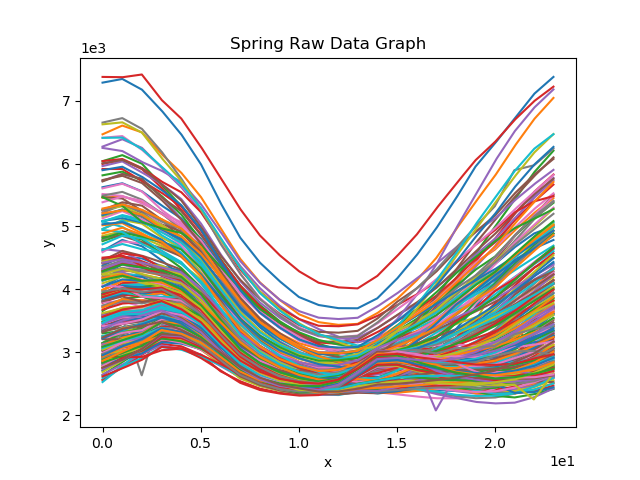
\includegraphics[height=1.8in]{Spring_Raw_Data_Graph_line.png}
        \caption{Raw \ac{aps} Spring Demand Data. x is in hours (the 24 hours in a day). y is APS's electric demand in MWe.}
    \end{subfigure}
     \hfill
    \begin{subfigure}[t]{\textwidth}
        \centering
        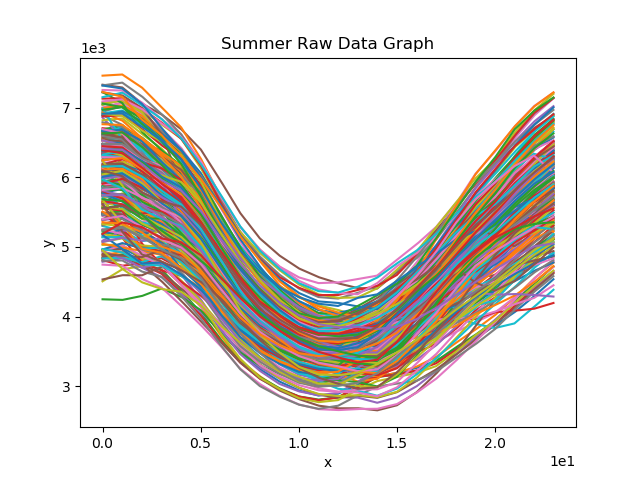
\includegraphics[height=1.8in]{Summer_Raw_Data_Graph_line.png}
        \caption{Raw \ac{aps} Summer Demand Data. x is in hours. y is APS's electric demand in MWe.}
    \end{subfigure}
    \vskip\baselineskip
    \begin{subfigure}[t]{\textwidth}
        \centering
        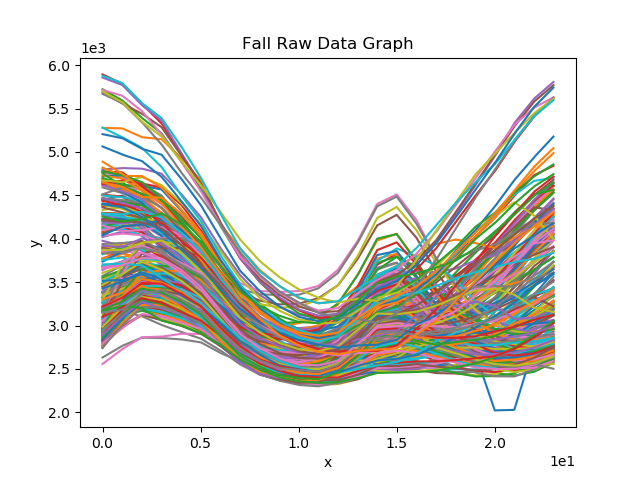
\includegraphics[height=1.8in]{Fall_Raw_Data_Graph_line.png}
        \caption{Raw \ac{aps} Fall Demand Data. x is in hours. y is APS's electric demand in MWe.}
    \end{subfigure}
    \quad
    \begin{subfigure}[t]{0.9\textwidth}
        \centering
        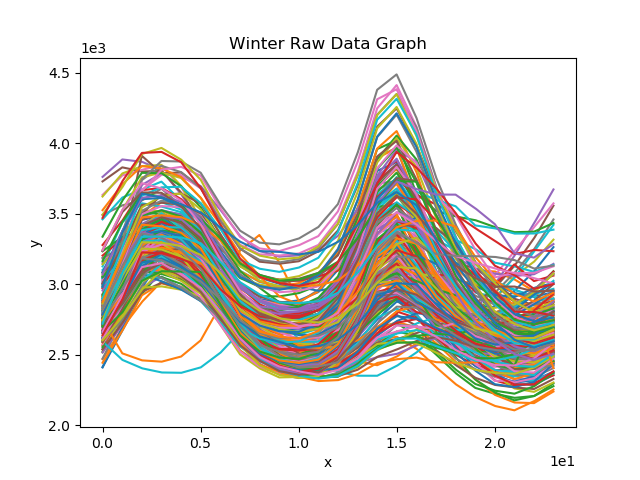
\includegraphics[height=1.8in]{Winter_Raw_Data_Graph_line.png}
        \caption{Raw \ac{aps} Winter Demand Data. x is in hours. y is APS's electric demand in MWe.}
    \end{subfigure}
        \label{RawDemand}
    \caption{Raw Data showing general Arizona Public Service Demand from the EIA from July 1st, 2015 to May 18, 2018}
\end{figure*}

\begin{figure*}[t!]
    \centering
    \label{SyntheticAverage}
    \begin{subfigure}[b]{0.9\textwidth}
        \centering
        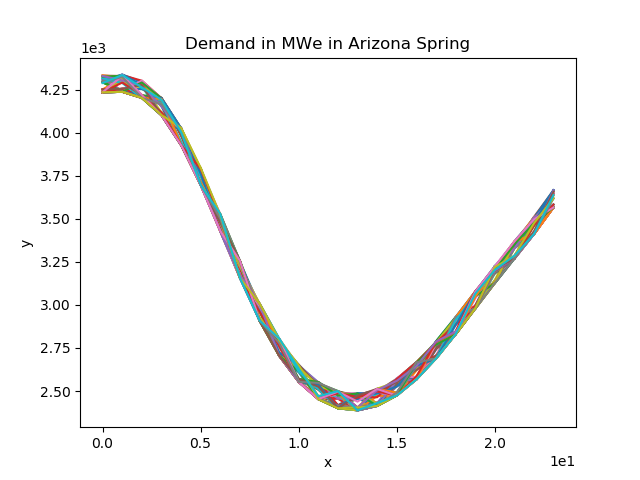
\includegraphics[height=1.8in]{Demand_in_MWe_in_Arizona_Spring_line.png}
        \caption{Spring \ac{aps} Demand Data. x is in hours (the 24 hours in a day). y is APS's electric demand in MWe.}
    \end{subfigure}
     \hfill
    \begin{subfigure}[t]{0.9\textwidth}
        \centering
        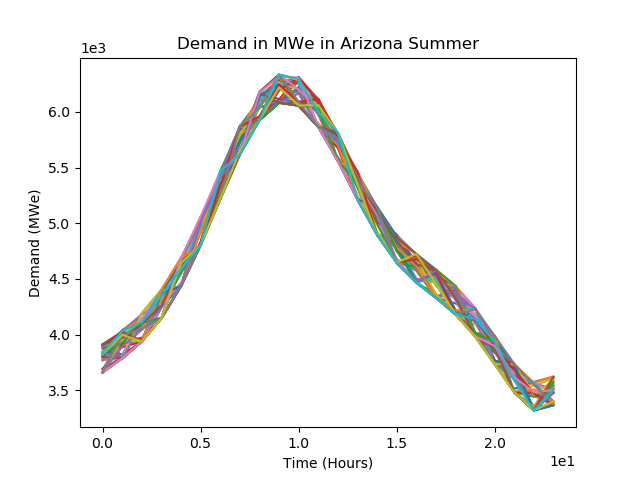
\includegraphics[height=1.8in]{Demand_in_MWe_in_Arizona_Summer_line.png}
        \caption{Synthetic \ac{aps} Summer Demand Data. x is in hours. y is APS's electric demand in MWe.}
    \end{subfigure}
    \vskip\baselineskip
    \begin{subfigure}[t]{0.9\textwidth}
        \centering
        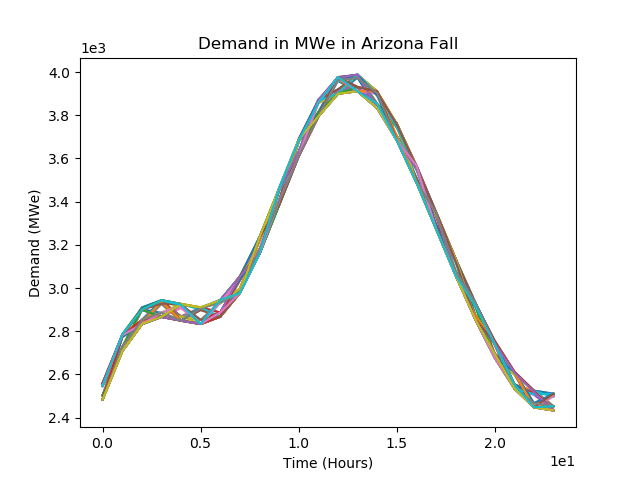
\includegraphics[height=1.8in]{Demand_in_MWe_in_Arizona_Fall_line.png}
        \caption{Synthetic \ac{aps} Fall Demand Data. x is in hours. y is APS's electric demand in MWe.}
    \end{subfigure}
    \quad
    \begin{subfigure}[t]{0.9\textwidth}
        \centering
        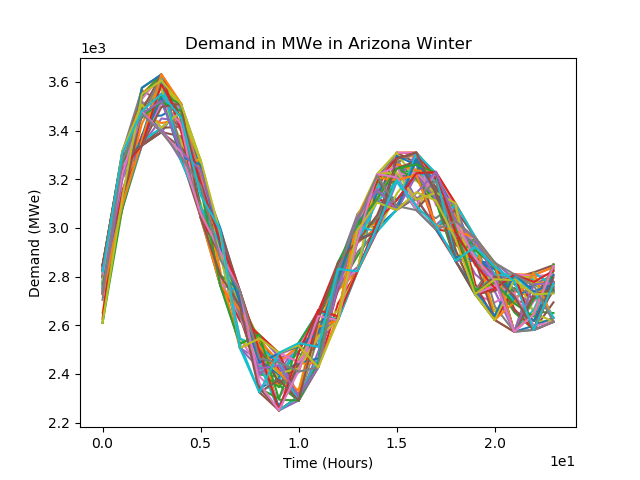
\includegraphics[height=1.8in]{Demand_in_MWe_in_Arizona_Winter_line.png}
        \caption{Synthetic \ac{aps} Winter Demand Data. x is in hours. y is APS's electric demand in MWe.}
    \end{subfigure}
    \caption{Cleaned up Synthetic Data showing general Arizona Public Service Demand}
\end{figure*}

\begin{table}[h!]
\centering
\caption{Approximate average values for demand change in Arizona over the four seasons}

\begin{tabular}{|l|l|l|l|l|l|}
\hline
\multicolumn{1}{|c|}{\textbf{Season}} & \multicolumn{1}{c|}{\textbf{\begin{tabular}[c]{@{}l@{}}Peak\\ Demand\\ (MWe)\end{tabular}}} & \textbf{\begin{tabular}[c]{@{}l@{}}Minimum\\ Demand\\ (MWe)\end{tabular}} & \textbf{\begin{tabular}[c]{@{}l@{}}Change in\\ Demand\\ (MWe)\end{tabular}} & \textbf{\begin{tabular}[c]{@{}l@{}}Local\\ Minimums\\ (MWe)\end{tabular}} & \textbf{\begin{tabular}[c]{@{}l@{}}Change in \\ Local\\Demand (MWe)\end{tabular}} \\ \hline
Spring                                & 4300                                      & 2320                                                              & 1980                                                                & N/A                                                               & N/A                                                                        \\ \hline
Summer                                & 6400                                      & 3500                                                              & 2900                                                                & N/A                                                               & N/A                                                                        \\ \hline
Fall                                  & 3900                                      & 2350                                                              & 1550                                                                & 2950                                                              & 950                                                                        \\ \hline
Winter                                & 3500                                      & 2450                                                              & 1050                                                                & 2500                                                              & 1000                                                                       \\ \hline
\end{tabular}
\label{DemandChange}
\end{table}

\subsection{Fluctuation Analysis}

As determined by the RAVEN assessment shown in table 3.12, the power shifts currently required due solely to changes in demand are greater than the amount of power APS owns from Palo Verde for all months besides winter.  If APS chooses to use Palo Verde as a major tool for load following, it would be most helpful to shift most of the load to uses other than the grid for portions of the day.  Clearly, as shown in figures 3.8 and 3.9, the transition from maximum electric demand to minimum electric demand is not a sharp drop off at one point in the day, but more of a gradual transition.

As the graphs and table \ref{DemandChange} demonstrate, the load change over a day would generally require that all of the electricity be diverted from the APS-owned load from Palo Verde.  Since the demand curves typically decrease and increase over several hours, the load would have to be shifted to water production in portions over the day if load following just with Palo Verde.  The various exergy and revenue outcomes from the thermally and electrically coupled systems at different rates of load following have already been detailed in tables \ref{LoadFollow}, \ref{SW-S}, \ref{SW-L}, and \ref{SW-M}. The tendency for the demand to shift gradually would suggest a benefit to electrically coupling, which does not have thermalhydraulic feedbacks from shifting.
% * <r.angelo.borrelli@gmail.com> 2018-06-12T23:34:11.313Z:
% 
% > As the graphs and table \ref{DemandChange} demonstrate, the load change over a day would generally require that all of the electricity be diverted from the APS-owned load from Palo Verde.  Since the demand curves typically decrease and increase over several hours, the load would have to be shifted to water production in portions over the day if load following just with Palo Verde.  The various exergy and revenue outcomes from the thermally and electrically coupled systems at different rates of load following have already been detailed in tables \ref{LoadFollow}, \ref{SW-S}, \ref{SW-L}, and \ref{SW-M}. The tendency for the demand to shift gradually would suggest a benefit to electrically coupling, which does not have thermalhydraulic feedbacks from shifting.
% So are you saying load following with Palo Verde alone would be inadequate? I feel like this is an important result, and I just want to make sure this passage is clear and direct. 
% 
% ^.


